\documentclass{beamer}
\usepackage{listings}
\lstset{
%language=C,
frame=single,
breaklines=true,
columns=fullflexible
}
\usepackage{subcaption}
\usepackage{url}
\usepackage{tikz}
\usepackage{tkz-euclide} % loads  TikZ and tkz-base
%\usetkzobj{all}
\usetikzlibrary{calc,math}
\usepackage{float}
\newcommand\norm[1]{\left\lVert#1\right\rVert}
\newcommand{\myvec}[1]{\ensuremath{\begin{pmatrix}#1\end{pmatrix}}}
\renewcommand{\vec}[1]{\mathbf{#1}}
\usepackage[export]{adjustbox}
\usepackage[utf8]{inputenc}
\usepackage{amsmath}
\usetheme{Boadilla}

\title{Challenging Problem 13}
\author{Perambuduri Srikaran}
\institute{IITH AI}
\date{June 6, 2021}
\begin{document}
\providecommand{\pr}[1]{\ensuremath{\Pr\left(#1\right)}}
\providecommand{\qfunc}[1]{\ensuremath{Q\left(#1\right)}}
\providecommand{\sbrak}[1]{\ensuremath{{}\left[#1\right]}}
\providecommand{\lsbrak}[1]{\ensuremath{{}\left[#1\right.}}
\providecommand{\rsbrak}[1]{\ensuremath{{}\left.#1\right]}}
\providecommand{\brak}[1]{\ensuremath{\left(#1\right)}}
\providecommand{\lbrak}[1]{\ensuremath{\left(#1\right.}}
\providecommand{\rbrak}[1]{\ensuremath{\left.#1\right)}}
\providecommand{\cbrak}[1]{\ensuremath{\left\{#1\right\}}}
\providecommand{\lcbrak}[1]{\ensuremath{\left\{#1\right.}}
\providecommand{\rcbrak}[1]{\ensuremath{\left.#1\right\}}}
\begin{frame}
\titlepage
\end{frame}
\section{Question}
\begin{frame}
\frametitle{Question}
\begin{block}{}
If each element of an $n^{th}$ order determinant is either 0 or 1, what is the probability that the value of the determinant is positive?\\
(Assume that the individual entries of the determinant are chosen independently, each value being assumed with probability $\frac{1}{2}$)
\end{block}
\end{frame}
\section*{Solution}
\begin{frame}[fragile]
\frametitle{Solution}
\begin{flushleft}
We will compute the number of invertible matrices. Let $a_{ij}$ represent the element in $i^{th}$ row and $j^{th}$ column.
\begin{align}
    \myvec{M}=
    \begin{bmatrix}
    a_{11} & \dots & a_{1n} \\
    \vdots & \ddots & \\
    a_{n1} &        & a_{nn}
    \end{bmatrix}
\end{align}
\begin{align}
    \myvec{v_i} =
    \begin{bmatrix}
    a_{i1} & \dots &a_{in}
    \end{bmatrix}
\end{align}
\end{flushleft}
\end{frame}
\begin{frame}[fragile]
\frametitle{Solution (contd...)}
\begin{flushleft}
Let $0_{1 \times n}$ represent row zero vector.
\begin{align}
    \pr{v_1 \neq 0_{1 \times n}} &= \frac{2^n - 1}{2^n}\\
    \pr{k_1v_1 + k_2v_2 \neq 0 | v_1 \neq 0_{1 \times n}} &= \frac{2^n - 2^1}{2^n}\\
    \pr{l_1v_1 + l_2v_2 + l_3v_3 \neq 0 | k_1v_1 + k_2v_2 \neq 0} &= \frac{2^n - 2^2}{2^n}
\end{align}
Similarly, we can find the probability of representing the row vectors.
\begin{align}
    \pr{\det{M} \neq 0} = \brak{1 - 2^{-1}}\brak{1 - 2^{-2}}\brak{1 - 2^{-3}}\dots\brak{1 - 2^{-n}}
\end{align}
\end{flushleft}
\end{frame}
\begin{frame}[fragile]
\frametitle{Solution (contd...)}
\begin{flushleft}
Matrices with $\det M < 0$ are the matrices resulting from swapping of first 2 rows of matrices with $\det M > 0$.
\begin{align}
    \pr{\det{M} > 0} &= \pr{\det{M} < 0}\\
    &= \frac{1}{2}\pr{\det{M} \neq 0}\\
    &= \frac{1}{2}\prod_{k=1}^{n}\brak{1 - 2^{-k}}
\end{align}
\end{flushleft}
\end{frame}
\begin{frame}[fragile]
\frametitle{Simulation}
\begin{flushleft}
\begin{figure}[h]
    \centering
    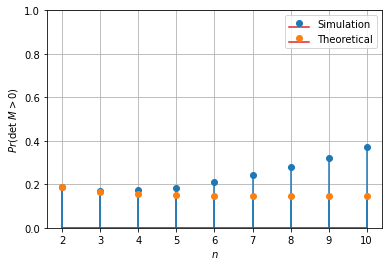
\includegraphics[width=8cm]{Fig2.png}
    \caption{Plot for Simulation v/s Theoretical}
    \label{fig:plot}
\end{figure}
\end{flushleft}
\end{frame}
\end{document}
